\section{Visão Computacional}
\label{sec:visao_comp}

A visão computacional está em constante avanço, aproximando cada vez mais os computadores da capacidade visual humana. De acordo com Horst Haußecker e Bernd Jähne, no livro "Computer Vision and Applications" \cite{comp_vision_and_applications}, a visão computacional é uma área da computação dedicada à interpretação de imagens por meio de algoritmos e técnicas de processamento de imagens. Essa área abrange a aquisição, processamento e análise de imagens, com o objetivo de extrair informações úteis para resolver problemas específicos.

Segundo Richard Szeliski no livro "Computer Vision: Algorithms and Applications" \cite{computer_vision_richard}, nas últimas décadas ocorreram avanços significativos na busca por aproximar a visão computacional da visão humana, porém não obteve total êxito. Isso ocorre porque, enquanto o olho humano enxerga com aparente facilidade as estruturas tridimensionais e suas nuances, enquanto visão computacional depende de técnicas matemáticas altamente precisas para recuperar a forma tridimensional e a aparência dos objetos.

Nas figuras \cref{fig:imagem_a} e \cref{fig:imagem_b}, evidencia-se a notável capacidade de um computador em distinguir, classificar e até mesmo compreender os elementos presentes em uma fotografia.

\begin{figure}[ht]
    \centering
    \begin{minipage}[h]{0.49\textwidth}
      \caption{Algoritmos de detecção facial e de roupas/cabelos por cor localizam e reconhecem pessoas nesta imagem}
      \centering
      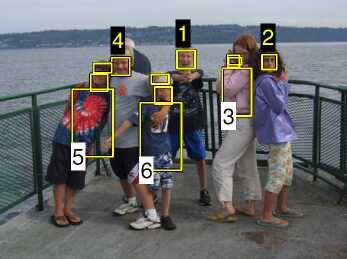
\includegraphics[width=0.6\textwidth]{figures/detectacao_de_faces_exemplo.JPG}
      \legend{Fonte: \citeonline{computer_vision_richard}}
      \label{fig:imagem_a}
    \end{minipage}
    \hfill
    \begin{minipage}[h]{0.49\textwidth}
      \caption{Segmentação de instâncias de objetos pode-se delinear cada pessoa e objeto em uma cena complexa}
      \centering
      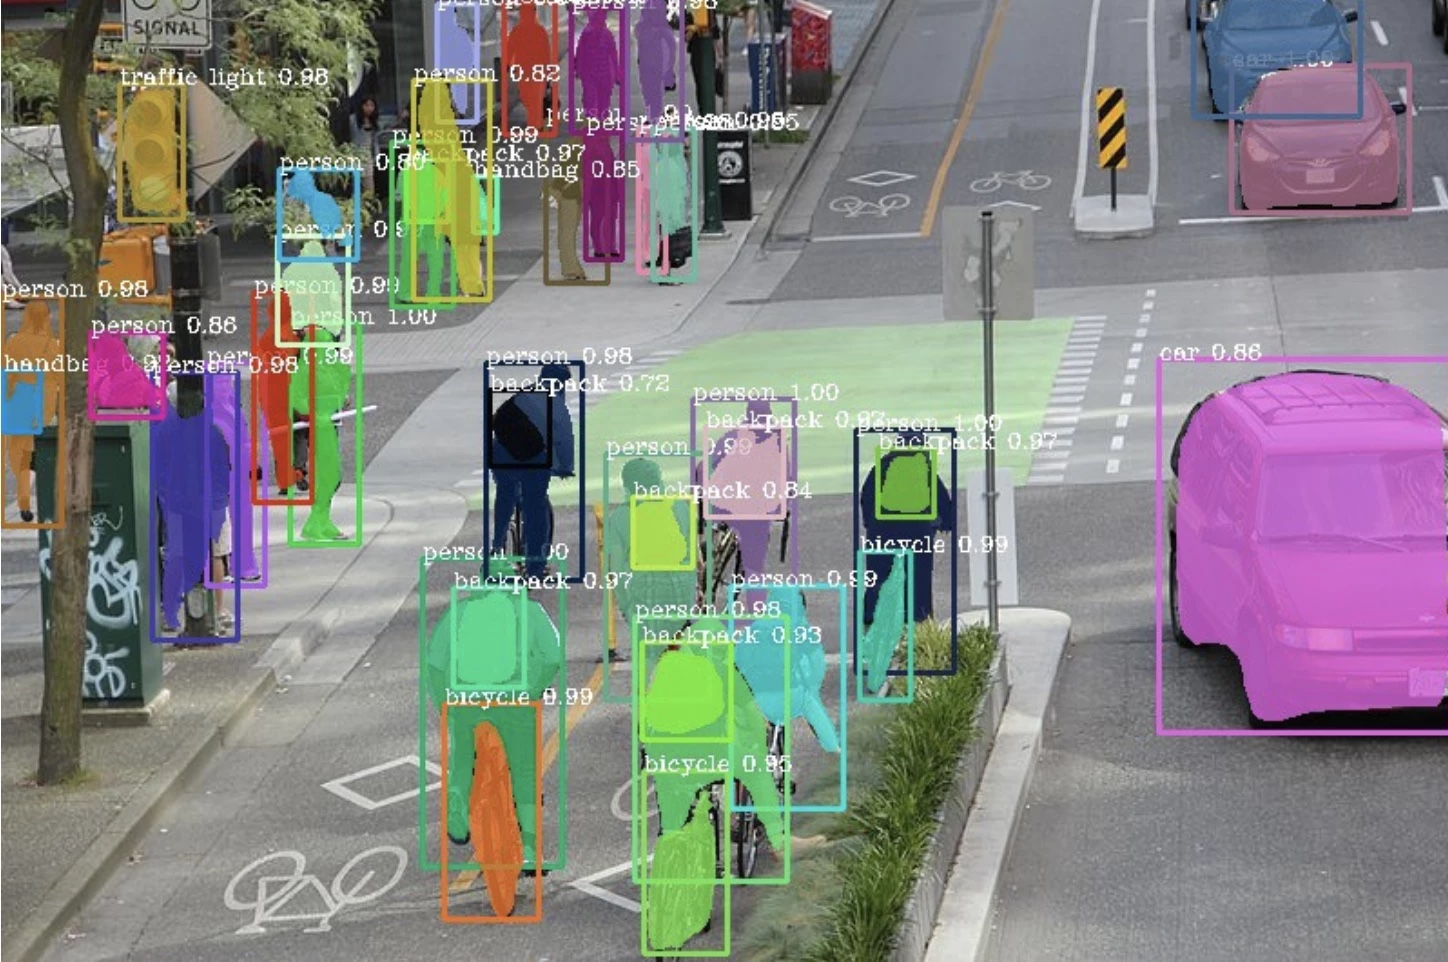
\includegraphics[width=0.6\textwidth]{figures/semantic_intance.JPG}
      \legend{Fonte: \citeonline{instance_segmentation}}
      \label{fig:imagem_b}
    \end{minipage}
\end{figure}

No entanto, apesar do sucesso no uso dessas técnicas, o computador ainda não consegue oferecer a mesma quantidade de detalhes na explicação de uma imagem como o olho humano. Isso se deve à maior facilidade do computador em compreender linguagem em comparação à visualização. A tarefa de ensinar um computador a ver e descrever com precisão e riqueza de detalhes o que está sendo observado é extremamente complexa \cite{computer_vision_richard}.

A visão é um elemento crucial para capacitar a inteligência artificial a realizar diversas tarefas. A fim de replicar a visão humana, é necessário que as máquinas sejam capazes de adquirir, processar, analisar e compreender imagens \cite{como_funciona_visao_computacional}.

No processamento de computação visual, as imagens são adquiridas e representadas como uma matriz 2D de píxeis. Cada pixel corresponde a um ponto na imagem e é representado por um valor numérico que varia de 0 a 255. Esses valores de pixel descrevem a intensidade da cor em uma escala de cinza, caso a imagem de entrada esteja em preto e branco, pois se a imagem ter cores do espectro RGB o computador identificará três matrizes de canais referentes às cores correspondentes. Dessa forma, um computador interpreta uma imagem como uma ou mais matrizes de números, permitindo que seja analisado e compreendido os detalhes visuais presentes na imagem. Um exemplo dessa matriz é exemplificado na \cref{fig:comp_vision} do presidente dos Estados Unidos, Abraham Lincoln \cite{mit_video}.

\begin{figure}[ht]
    \caption{Diagrama de dados de píxeis. À esquerda, uma imagem de Lincoln; no centro, os píxeis rotulados com números de 0 a 255, representando sua luminosidade; e à direita, apenas esses números.}
    \centering
    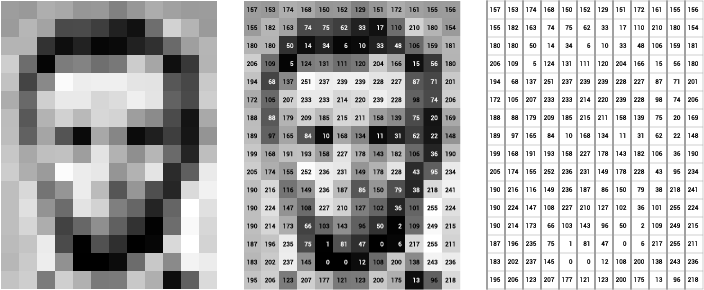
\includegraphics[width=0.6\textwidth]{figures/lincoln_pixel_values.png}
    \legend{Fonte: \citeonline{content_Human_Vision}}
    \label{fig:comp_vision}
\end{figure}

Os algoritmos de visão computacional utilizados atualmente são fundamentados em reconhecimento de padrões. O procedimento consiste em treinar computadores por meio de uma vasta quantidade de dados visuais. Os computadores processam imagens, rotulam os objetos nelas contidos e identificam padrões entre esses objetos \cite{content_Human_Vision}.

Esse processo de treinamento e reconhecimento de padrões permite que os computadores identifiquem objetos e compreendam seu contexto visual. Com essa capacidade, o computador consegue realizar tarefas como, por exemplo, reconhecimento facial, como na \cref{fig:imagem_a}.

Em visão computacional, é comum usar algumas técnicas para separar objetos de interesse, pois a partir disso é possível aplicar alterações em objetos específicos, e para isso, utiliza-se uma técnica chamada de máscara binária \cite{NVIDIA,Embarcados}.

A máscara binária — ou imagem binária — contém apenas duas cores, geralmente preto e branco, ou valores 0 e 1. Sendo o branco (ou 1) o objeto em destaque e o preto (ou 0) o fundo \cite{Embarcados}.

Serão abordados dois algoritmos com propostas parecidas para selecionar um objeto e destacá-lo em uma imagem binária, sendo eles: selecionar imagem por cor e por inundação. Ambos utilizam a biblioteca em Python, OpenCV, uma biblioteca multiplataforma para visão computacional, com métodos para auxiliar na manipulação, por exemplo, de imagens \cite{OpenCV}.

O método de selecionar por cor fundamenta-se em capturar a cor específica do clique na imagem e percorrer a imagem comparando a cor alvo com a cor da imagem. Caso seja a mesma, pinte o mesmo pixel da nova imagem como branco; caso não seja, pinte como preto. Uma maneira performática de selecionar por cor é definir um espectro de cores e aplicar uma máscara usando o método \textit{inRange} da biblioteca OpenCV; pode-se escolher apenas uma cor \cite{OpenCVInRange}.

O método de selecionar por preenchimento por inundação é um algoritmo de expansão a partir de um pixel, validando se contém a mesma cor. A implementação inicia uma matriz de zeros com tamanho 2 pixels maior do que a imagem original. O clique na imagem será a semente — ou em inglês, seed — e a partir disso o algoritmo começa uma expansão para os pixels vizinhos — de cima, baixo, esquerda e direita — caso contenha a mesma cor, pinta de branco, e refaz com os pixels marcados anteriormente até não ter mais pontos brancos para marcar \cite{OpenCVFloodFill}.

Ademais, existem diversas opções de ferramentas que auxiliam na criação de interfaces gráficas para visualização e manipulação de imagens, fornecendo funções e modelos para criar telas, sendo uma das mais utilizadas o PyQt5 \cite{uniteai2023}.

\subsection{PyQt5}

O PyQt5 incorpora as bibliotecas Qt em C++, proporcionando recursos para o desenvolvimento multiplataforma. Isso simplifica a criação de interfaces em Python em diversos ambientes, como Windows, Mac, Linux e dispositivos móveis \cite{pyqt5}.
